实现五级流水cpu的过程主要参考《自己动手写CPU》\cite{book}。
\subsection{实现功能}
\subsubsection{指令集}
在实现的过程中,实际实现了下列指令: \\
and, or, xor, nor, andi, ori, xori, lui, sll, sllv, sra, srav, srl, srlv, \\
movn, movz. mfhi, mthi, mflo, mtlo, \\
add, addu, sub, subu, slt, sltu, addi, addiu, \\
slti, sltiu, clo, clz, \\
multu, mult, mul, \\
jr, jalr, j, jal, \\
j, jr, beq, bne, \\
lb, lw, sb, sw
\subsubsection{其他结构}
为了防止Hazards,通过ctrl模块实现了流水线的暂停。同时通过实现forwarding来避免数据相关。


\subsection{大致结构}
	实现的模块和大致结构如下图(仅ori指令): \\
	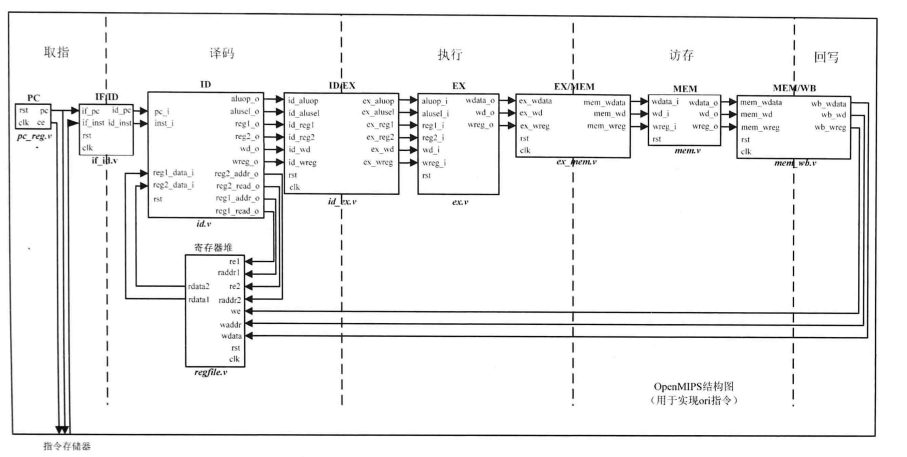
\includegraphics[width = 400]{Picture1.png}
	之后为了实现其他指令、forwarding、流水线stall等陆续添加了其他若干接口。

\subsection{代码实现模块}
	在代码上,实现了这些模块:
	% 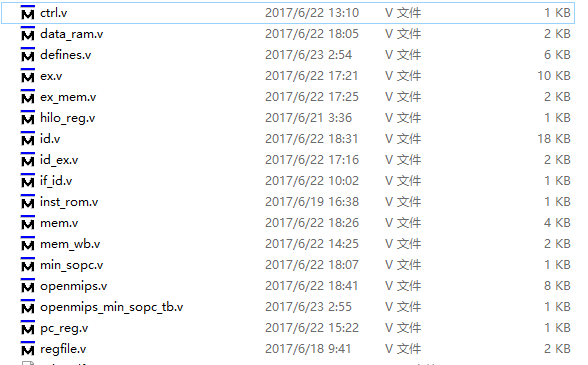
\includegraphics[width = 400]{Picture2.png}
	\subsubsection*{PC}
	给出指令地址。
	\subsubsection*{IF-ID}
	暂时保存取指令阶段取得的指令,以及对应的指令地址,并在下一个时钟传递到译码阶段。
	\subsubsection*{Regfile}
	实现了$32$个$32$位通用整数寄存器,可以同时进行两个寄存器的读操作和一个寄存器的写操作。
	\subsubsection*{ID}
	对指令进行译码,得到最终运算的类型、子类型、源操作数、目的寄存器地址等信息。
	\subsubsection*{ID-EX}
	将译码阶段取得的结果在下一个时钟传递到流水线执行阶段。
	\subsubsection*{EX}
	根据获得的数据进行运算。
	\subsubsection*{EX-MEM}
	将执行阶段取得的结果在下一个时钟传递到流水线访存阶段。
	\subsubsection*{MEM}
	访问数据储存器RAM。
	\subsubsection*{MEM-WB}
	将访存阶段取得的结果在下一个时钟传递到流水线回写阶段。
	\subsubsection*{RAM}
	实现了4个按字节寻址的8位储存器。
	\subsubsection*{MIPS}
	对各个模块进行实例化,按照链接关系图链接。

\subsection{遇到的问题}
ModelSim软件运行比较慢。而且没有找到除了直接看代码之外比较有效率的调试方法。\\
由于是模拟硬件运行,很多规则都是自己规定,在体系结构对于运算速度的影响上缺少一些直观感受。

\subsection{正确性验证方法}
首先,《自己动手写CPU》\cite{book} 中对于不同类型的指令都给出了测试程序,测试这些程序后波形与预期一致。 \\
其次,通过了郑怜悯同学构造的数据。 \\
所以,本人实现的代码应该基本正确。

\subsection{关于FPGA}
作业中的bonus项(在FPGA上实现cpu)没有完成。之前的部分代码不算太多但调试花费的时间太多,在ddl之前没有足够的时间学习和实现FPGA的使用。
